\chapter{CƠ SỞ LÝ THUYẾT}\label{Chapter2}

\section*{Tóm tắt chương}

Chương này trình bày các nền tảng kỹ thuật cần thiết cho khóa luận: IDS, dữ liệu lưu lượng mạng, DL cho IDS, FL, chắt lọc tri thức, FD, CIL và các thuật toán được dùng trong hệ thống. Trọng tâm của chương là các khái niệm phục vụ giải thích trực tiếp cho hệ thống FD phi tập trung kết hợp CIL.

\section{Hệ thống phát hiện xâm nhập}

\subsection{Tổng quan}

IDS là thành phần giám sát được đặt trong hệ thống mạng hoặc trên máy chủ nhằm theo dõi hành vi đang diễn ra và phát hiện dấu hiệu xâm nhập. Nếu tường lửa quyết định luồng nào được phép đi qua dựa trên chính sách truy cập, IDS quan sát phần lưu lượng và hoạt động đã đi vào hệ thống để nhận diện những biểu hiện bất thường. Vì vậy, IDS không thay thế cơ chế kiểm soát truy cập, mà bổ sung một lớp nhận biết sau kiểm soát, nơi những kết nối hợp lệ về mặt cổng, giao thức hoặc quyền truy cập vẫn có thể được phân tích sâu hơn về nội dung và mẫu hành vi.
\bigbreak\noindent
Trong khóa luận này, IDS được xem như một bài toán học từ dữ liệu lưu lượng mạng. Mỗi mẫu dữ liệu là một quan sát đã được biểu diễn bằng các đặc trưng như thời lượng phiên, số gói, số byte, hướng truyền, cổng, giao thức hoặc các thống kê theo luồng. Đầu ra của mô hình có thể là cảnh báo nhị phân hoặc nhãn đa lớp, nhưng bối cảnh CICIoT2023 yêu cầu phân loại chi tiết hơn giữa nhiều họ tấn công. Cách nhìn đa lớp này có giá trị vận hành rõ ràng hơn, vì một cảnh báo DDoS, một cảnh báo quét cổng và một cảnh báo SQL injection dẫn đến những hướng xử lý khác nhau.
\bigbreak\noindent
Theo cơ chế phát hiện, IDS thường được chia thành hai nhóm chính: dựa trên chữ ký (signature-based) và dựa trên bất thường (anomaly-based). IDS dựa trên chữ ký so khớp quan sát hiện tại với các mẫu tấn công đã biết, nhờ đó dễ kiểm tra và dễ giải thích nhưng phụ thuộc mạnh vào tri thức có sẵn. Ngược lại, IDS dựa trên bất thường học vùng hành vi bình thường hoặc vùng hành vi đã quan sát, sau đó đánh dấu những mẫu lệch khỏi vùng này. Hướng thứ hai phù hợp hơn khi tấn công thay đổi liên tục, nhưng cũng đòi hỏi mô hình có khả năng học bối cảnh thay vì chỉ dựa trên một vài ngưỡng đơn giản.
\bigbreak\noindent
Dữ liệu IDS có những đặc điểm khiến bài toán khó hơn phân loại thông thường. Phân phối lớp thường mất cân bằng, trong đó lưu lượng bình thường hoặc một vài nhóm tấn công lớn có thể áp đảo các lớp hiếm. Phân phối dữ liệu cũng thay đổi theo thời gian, vì hành vi mạng trong giờ cao điểm, giai đoạn cập nhật hệ thống hoặc thời điểm bị tấn công không giống nhau. Bên cạnh đó, cùng một kiểu tấn công có thể biểu hiện khác nhau giữa các miền mạng, khiến một mô hình học tốt ở tổ chức này chưa chắc hoạt động ổn định ở tổ chức khác. Những đặc điểm này là lý do IDS cần được đặt trong bối cảnh học phân tán, dữ liệu Non-IID và cập nhật tri thức liên tục.

\subsection{Hệ thống phát hiện xâm nhập dựa trên học máy}

IDS dựa trên học máy biến phát hiện xâm nhập thành bài toán học ánh xạ từ dữ liệu sang nhãn. Thay vì viết luật thủ công cho từng dạng tấn công, mô hình được huấn luyện trên các cặp mẫu và nhãn đã biết để tìm ra ranh giới phân loại trong không gian đặc trưng. Sau tiền xử lý, mỗi mẫu lưu lượng trở thành một vector số; mô hình nhận vector này, tạo dự đoán, so sánh với nhãn đúng và cập nhật tham số thông qua tối ưu mất mát. Quy trình này giúp quy tắc phân loại được hình thành từ dữ liệu, thay vì được mô tả trực tiếp bằng luật cố định.
\bigbreak\noindent
Với một vector đầu vào $x$, mô hình $f$ có tham số $w$ sinh logit $z=f(x;w)$ và xác suất lớp
$$
p_k(x)=\frac{\exp(z_k)}{\sum_j \exp(z_j)}.
$$
Nếu nhãn mục tiêu là $y$, hàm mất mát thường dùng là entropy chéo
$$
L_{cls}=-\frac{1}{N}\sum_{i=1}^{N}\sum_{k=1}^{K} y_{ik}\log p_k(x_i).
$$
Logit là điểm số thô trước khi chuyển thành xác suất, còn softmax biến các điểm số này thành phân phối trên các lớp. Entropy chéo phạt mô hình khi xác suất dành cho lớp đúng bị thấp. Trong IDS đa lớp, cơ chế này phù hợp vì mô hình phải cạnh tranh giữa nhiều khả năng tấn công cùng lúc, chẳng hạn một mẫu có thể gần DDoS hơn DoS hoặc gần reconnaissance hơn brute force.
\bigbreak\noindent
Đánh giá IDS dựa trên học máy không nên chỉ dựa vào accuracy. Với dữ liệu mất cân bằng, một mô hình có thể đạt accuracy cao bằng cách dự đoán tốt lớp lớn nhưng bỏ sót lớp nhỏ. Trong an ninh mạng, bỏ sót một lớp tấn công hiếm vẫn có thể gây hậu quả nghiêm trọng. Vì vậy, precision, recall và F1-score có vai trò quan trọng hơn trong nhiều tình huống. Với bài toán nhiều lớp như CICIoT2023, macro-F1 đặc biệt hữu ích vì chỉ số này đối xử các lớp công bằng hơn, không để lớp có nhiều mẫu áp đảo hoàn toàn kết quả đánh giá.
\bigbreak\noindent
Học máy cổ điển và DL đều có thể dùng cho IDS, nhưng DL phù hợp hơn khi dữ liệu lớn, quan hệ giữa đặc trưng phức tạp và mô hình cần học biểu diễn nhiều tầng. Các lớp đầu học biến đổi cơ bản của đặc trưng, các lớp giữa kết hợp đặc trưng thành mẫu trừu tượng hơn, còn lớp cuối chuyển biểu diễn đó thành quyết định phân loại. Đây là cơ sở để khóa luận dùng MLP, GRU và DCNN-BiLSTM như những đại diện cho các mức độ biểu diễn khác nhau.

\section{Học sâu cho hệ thống phát hiện xâm nhập}

\subsection{Multi Layer Perceptron}

Multi Layer Perceptron (MLP) là một kiến trúc mô hình phân loại cơ bản nhất cho dữ liệu dạng bảng. Đầu vào của mô hình là một vector đặc trưng đã được chuẩn hóa. Mỗi lớp dense thực hiện một phép biến đổi tuyến tính rồi đưa kết quả qua hàm kích hoạt phi tuyến (như ReLU hoặc Swish). Phép biến đổi tuyến tính kết hợp các đặc trưng đầu vào bằng trọng số học được, còn hàm kích hoạt giúp mô hình biểu diễn quan hệ phi tuyến. Nếu chỉ có các phép tuyến tính, nhiều lớp ghép lại vẫn tương đương một phép tuyến tính lớn. Chính hàm kích hoạt làm cho mạng dense học được các biên phân loại cong và phức tạp hơn.
\bigbreak\noindent
Trong lan truyền xuôi (forward pass), vector đặc trưng đi qua từng lớp theo thứ tự. Lớp đầu học các kết hợp đơn giản giữa đặc trưng, chẳng hạn quan hệ giữa số gói, số byte và thời lượng. Các lớp sau kết hợp tiếp những biểu diễn này để hình thành mẫu trừu tượng hơn. Với IDS, một đặc trưng riêng lẻ hiếm khi đủ kết luận tấn công. Nhưng tổ hợp nhiều đặc trưng có thể tạo dấu hiệu rõ hơn. Mạng dense phù hợp với tình huống này vì mỗi neuron ở một lớp có thể nhìn toàn bộ đầu ra của lớp trước, từ đó học tương tác giữa nhiều trường dữ liệu.
\bigbreak\noindent
Các thành phần phụ trong MLP cũng có vai trò riêng. Layer normalization ổn định phân phối kích hoạt giữa các lớp, giúp quá trình học ít dao động hơn khi đặc trưng có thang đo khác nhau. Dropout tắt ngẫu nhiên một phần kích hoạt trong huấn luyện, buộc mô hình không phụ thuộc quá mức vào một vài neuron và giảm overfitting. Kết nối dư giúp tín hiệu đi qua mạng dễ hơn bằng cách cộng biểu diễn cũ với biểu diễn mới. Điều này hỗ trợ lan truyền gradient, đặc biệt khi mạng có nhiều lớp. Lớp logits cuối cùng sinh ra một điểm số cho mỗi lớp, sau đó softmax chuyển điểm số thành xác suất dự đoán.
\bigbreak\noindent
Trong lan truyền ngược (backpropagation), mất mát (loss) từ đầu ra được truyền ngược qua softmax, lớp logits và các lớp dense trước đó. Mỗi trọng số được cập nhật theo hướng làm tăng xác suất của lớp đúng và giảm xác suất của lớp sai. Với dữ liệu IDS, quá trình này dần điều chỉnh các trọng số để mô hình nhận ra những tổ hợp đặc trưng gắn với từng lớp tấn công. Ưu điểm của MLP là tốc độ nhanh, ít giả định về thứ tự đặc trưng và dễ triển khai trên nhiều client. Hạn chế của nó là không khai thác trực tiếp cấu trúc tuần tự nếu dữ liệu có quan hệ theo thời gian hoặc theo thứ tự trường.

\subsection{Gated Recurrent Unit}

\begin{figure}[ht]
    \centering
    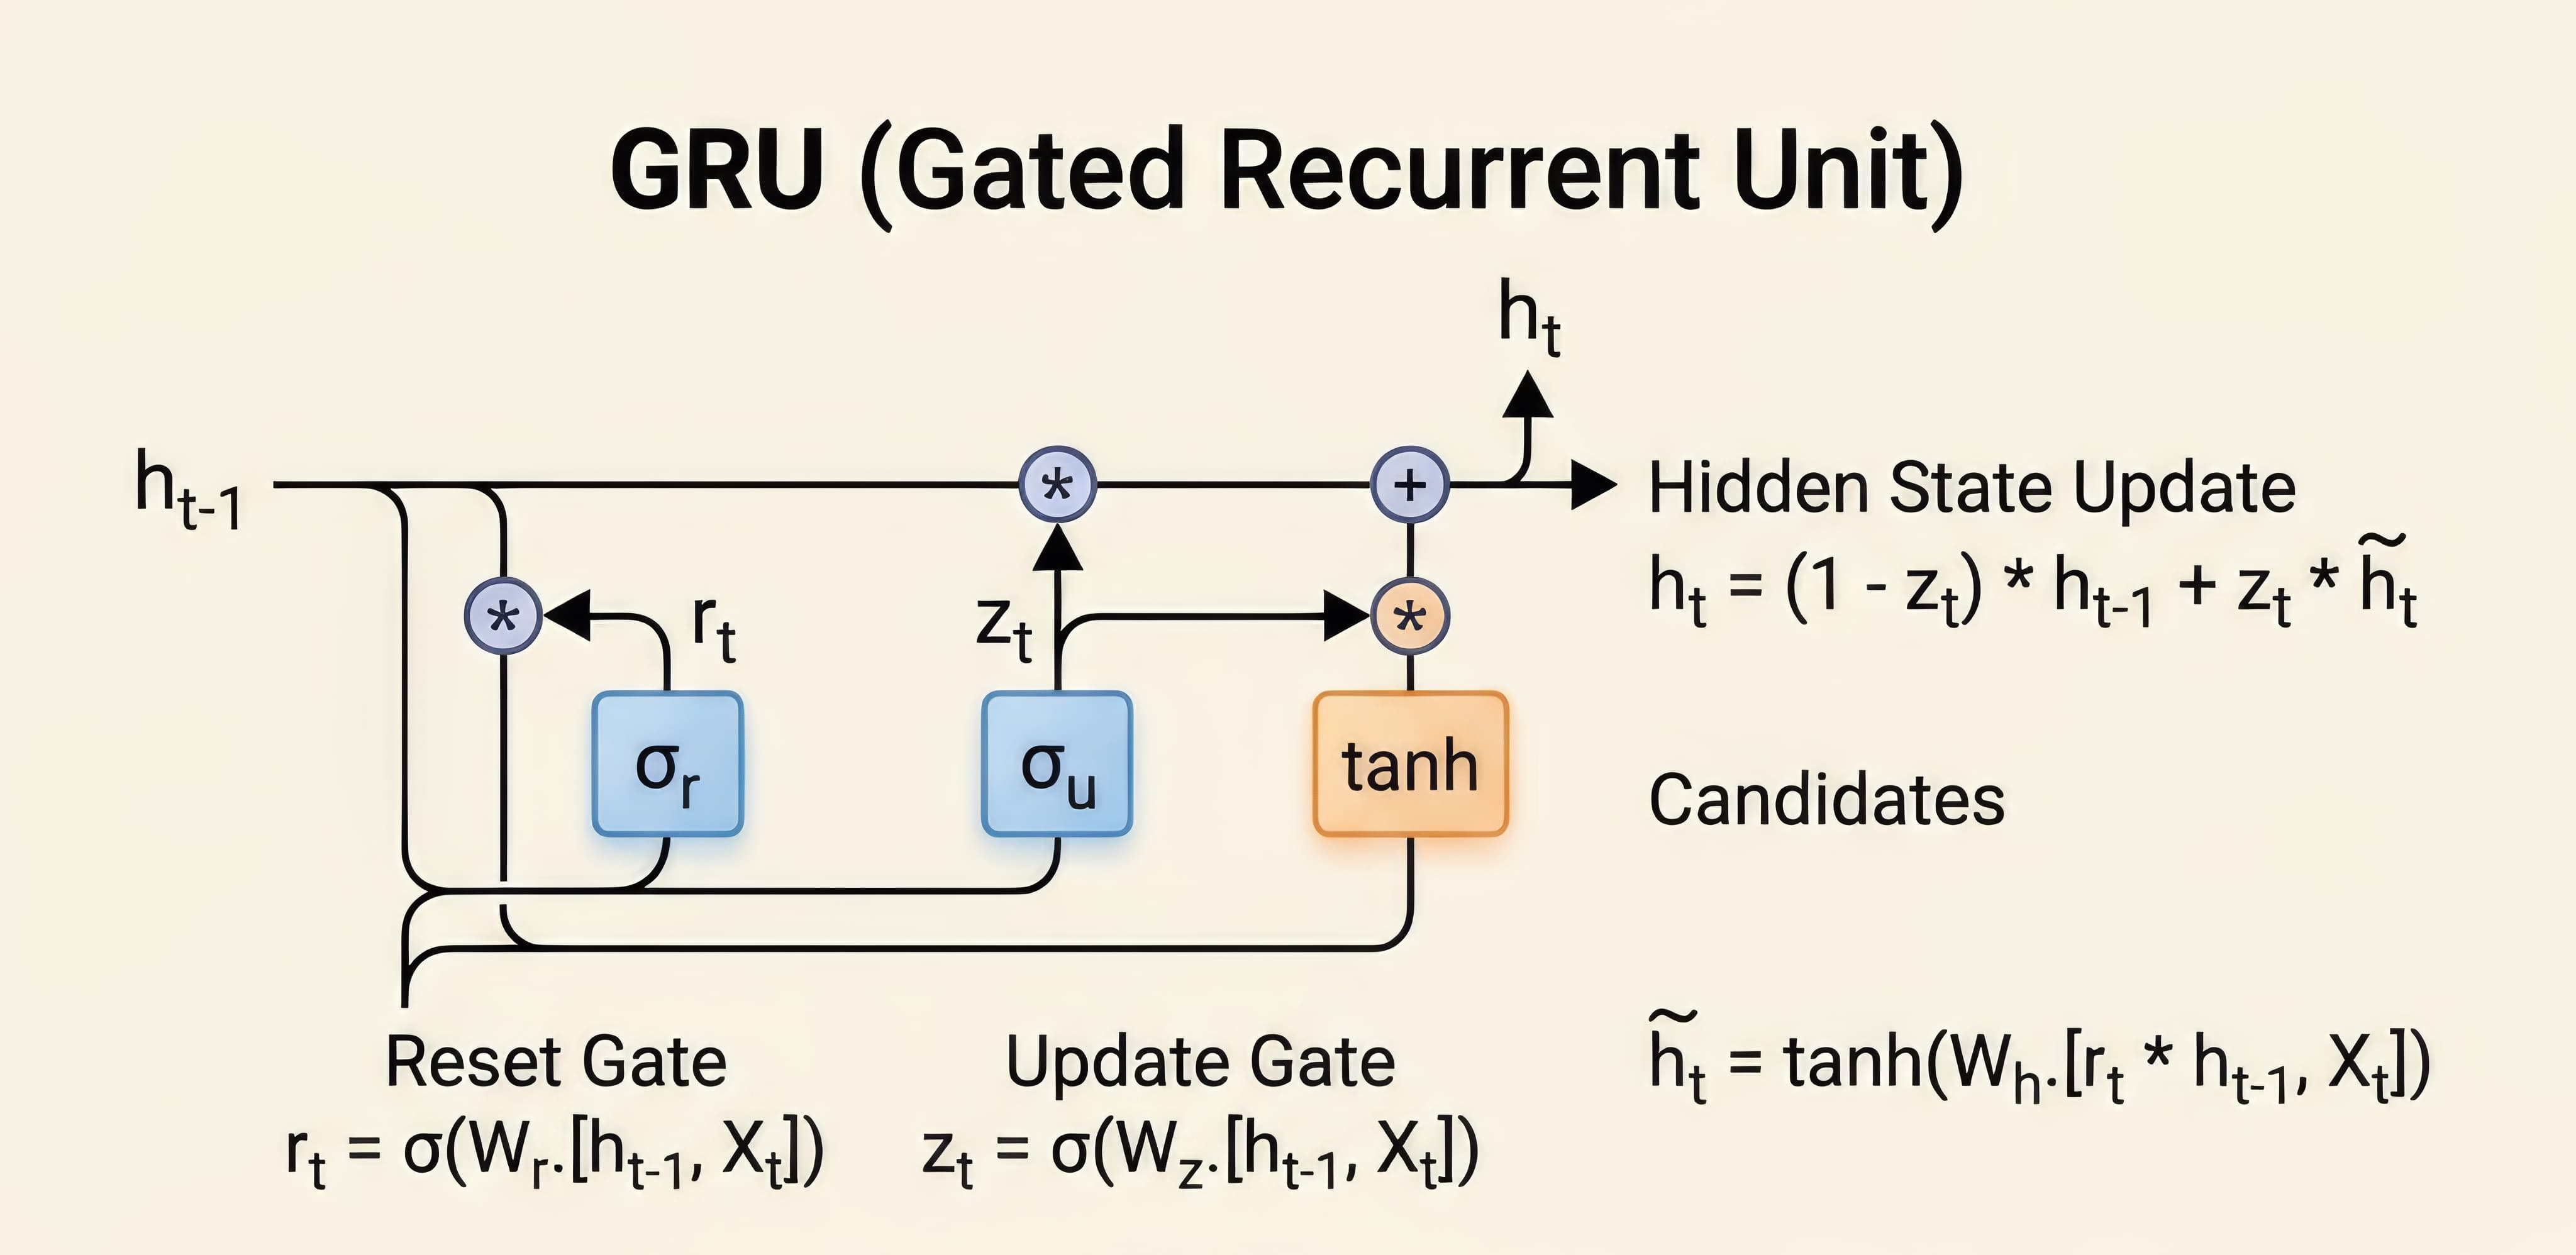
\includegraphics[width=0.8\textwidth]{images/GRU.jpg}
    \caption{Cấu trúc của GRU.}
\end{figure}

GRU là một kiến trúc mạng hồi tiếp được thiết kế để xử lý dữ liệu có cấu trúc chuỗi. Trong mô hình dùng cho IDS, vector đặc trưng có thể được tổ chức lại thành một chuỗi, trong đó mỗi đặc trưng được xem như một bước đầu vào. Cách nhìn này cho phép mô hình đọc dữ liệu tuần tự và duy trì một trạng thái ẩn trong quá trình đọc. Trạng thái ẩn đóng vai trò như bộ nhớ tóm tắt những gì mô hình đã thấy ở các bước trước.
\bigbreak\noindent
Điểm cốt lõi của GRU nằm ở hai cổng: cổng cập nhật (update gate) và cổng đặt lại (reset gate). Cổng cập nhật quyết định bao nhiêu thông tin cũ trong trạng thái ẩn cần được giữ lại khi đọc bước mới. Nếu thông tin cũ vẫn hữu ích, cổng này giữ bộ nhớ ổn định. Nếu bước mới mang tín hiệu quan trọng hơn, cổng cho phép trạng thái thay đổi mạnh hơn. Cổng đặt lại quyết định phần nào của trạng thái cũ nên được quên khi tính ứng viên trạng thái mới. Nhờ hai cổng này, GRU có thể cân bằng giữa ghi nhớ và cập nhật, tránh việc mọi bước đầu vào đều làm mất thông tin trước đó.
\bigbreak\noindent
Trong lan truyền xuôi, mẫu IDS đi qua các lớp GRU theo từng bước. Lớp GRU đầu tạo một chuỗi trạng thái ẩn, mỗi trạng thái phản ánh thông tin đã tích lũy đến vị trí tương ứng. Các lớp GRU tiếp theo tiếp tục đọc chuỗi biểu diễn này để học mẫu phức tạp hơn. Lớp GRU cuối thường trả về trạng thái cuối cùng, xem như bản tóm tắt toàn bộ chuỗi đặc trưng. Bản tóm tắt này đi qua một lớp dense để chuyển thành logits và xác suất lớp sau cùng. Với dữ liệu IDS, GRU có thể học các quan hệ có tính phụ thuộc thứ tự, chẳng hạn một nhóm đặc trưng chỉ có ý nghĩa khi xuất hiện cùng các đặc trưng đứng trước hoặc đứng sau nó.
\bigbreak\noindent
Trong quá trình tinh chỉnh trọng số mô hình, gradient được truyền ngược qua các bước thời gian của GRU. Cơ chế này thường được gọi là backpropagation through time (BPTT). Các cổng của GRU giúp gradient đi qua chuỗi ổn định hơn so với RNN đơn giản, vì mô hình có đường giữ trạng thái cũ và không buộc mọi thông tin phải được viết lại ở mỗi bước. So với LSTM, GRU có ít cổng hơn nên số tham số và chi phí tính toán thường thấp hơn. Điều này làm GRU phù hợp với client có tài nguyên hạn chế trong môi trường học liên kết, nơi mỗi client phải huấn luyện cục bộ nhiều vòng.
\bigbreak\noindent
Đối với dữ liệu IDS dạng bảng, GRU không phải lúc nào cũng vượt trội MLP, vì thứ tự đặc trưng không giống thứ tự thời gian tự nhiên trong văn bản hoặc tín hiệu. Tuy nhiên, GRU vẫn có giá trị khi cách sắp xếp đặc trưng mang thông tin hoặc khi muốn kiểm tra lợi ích của biểu diễn tuần tự. Trong ngữ cảnh mô hình không đồng nhất, GRU cũng đóng vai trò một kiến trúc trung gian: phức tạp hơn MLP, có khả năng ghi nhớ trạng thái, nhưng nhẹ hơn các mô hình lai DCNN-BiLSTM sâu hơn.

\subsection{DCNN-BiLSTM}

\begin{figure}[ht]
    \centering
    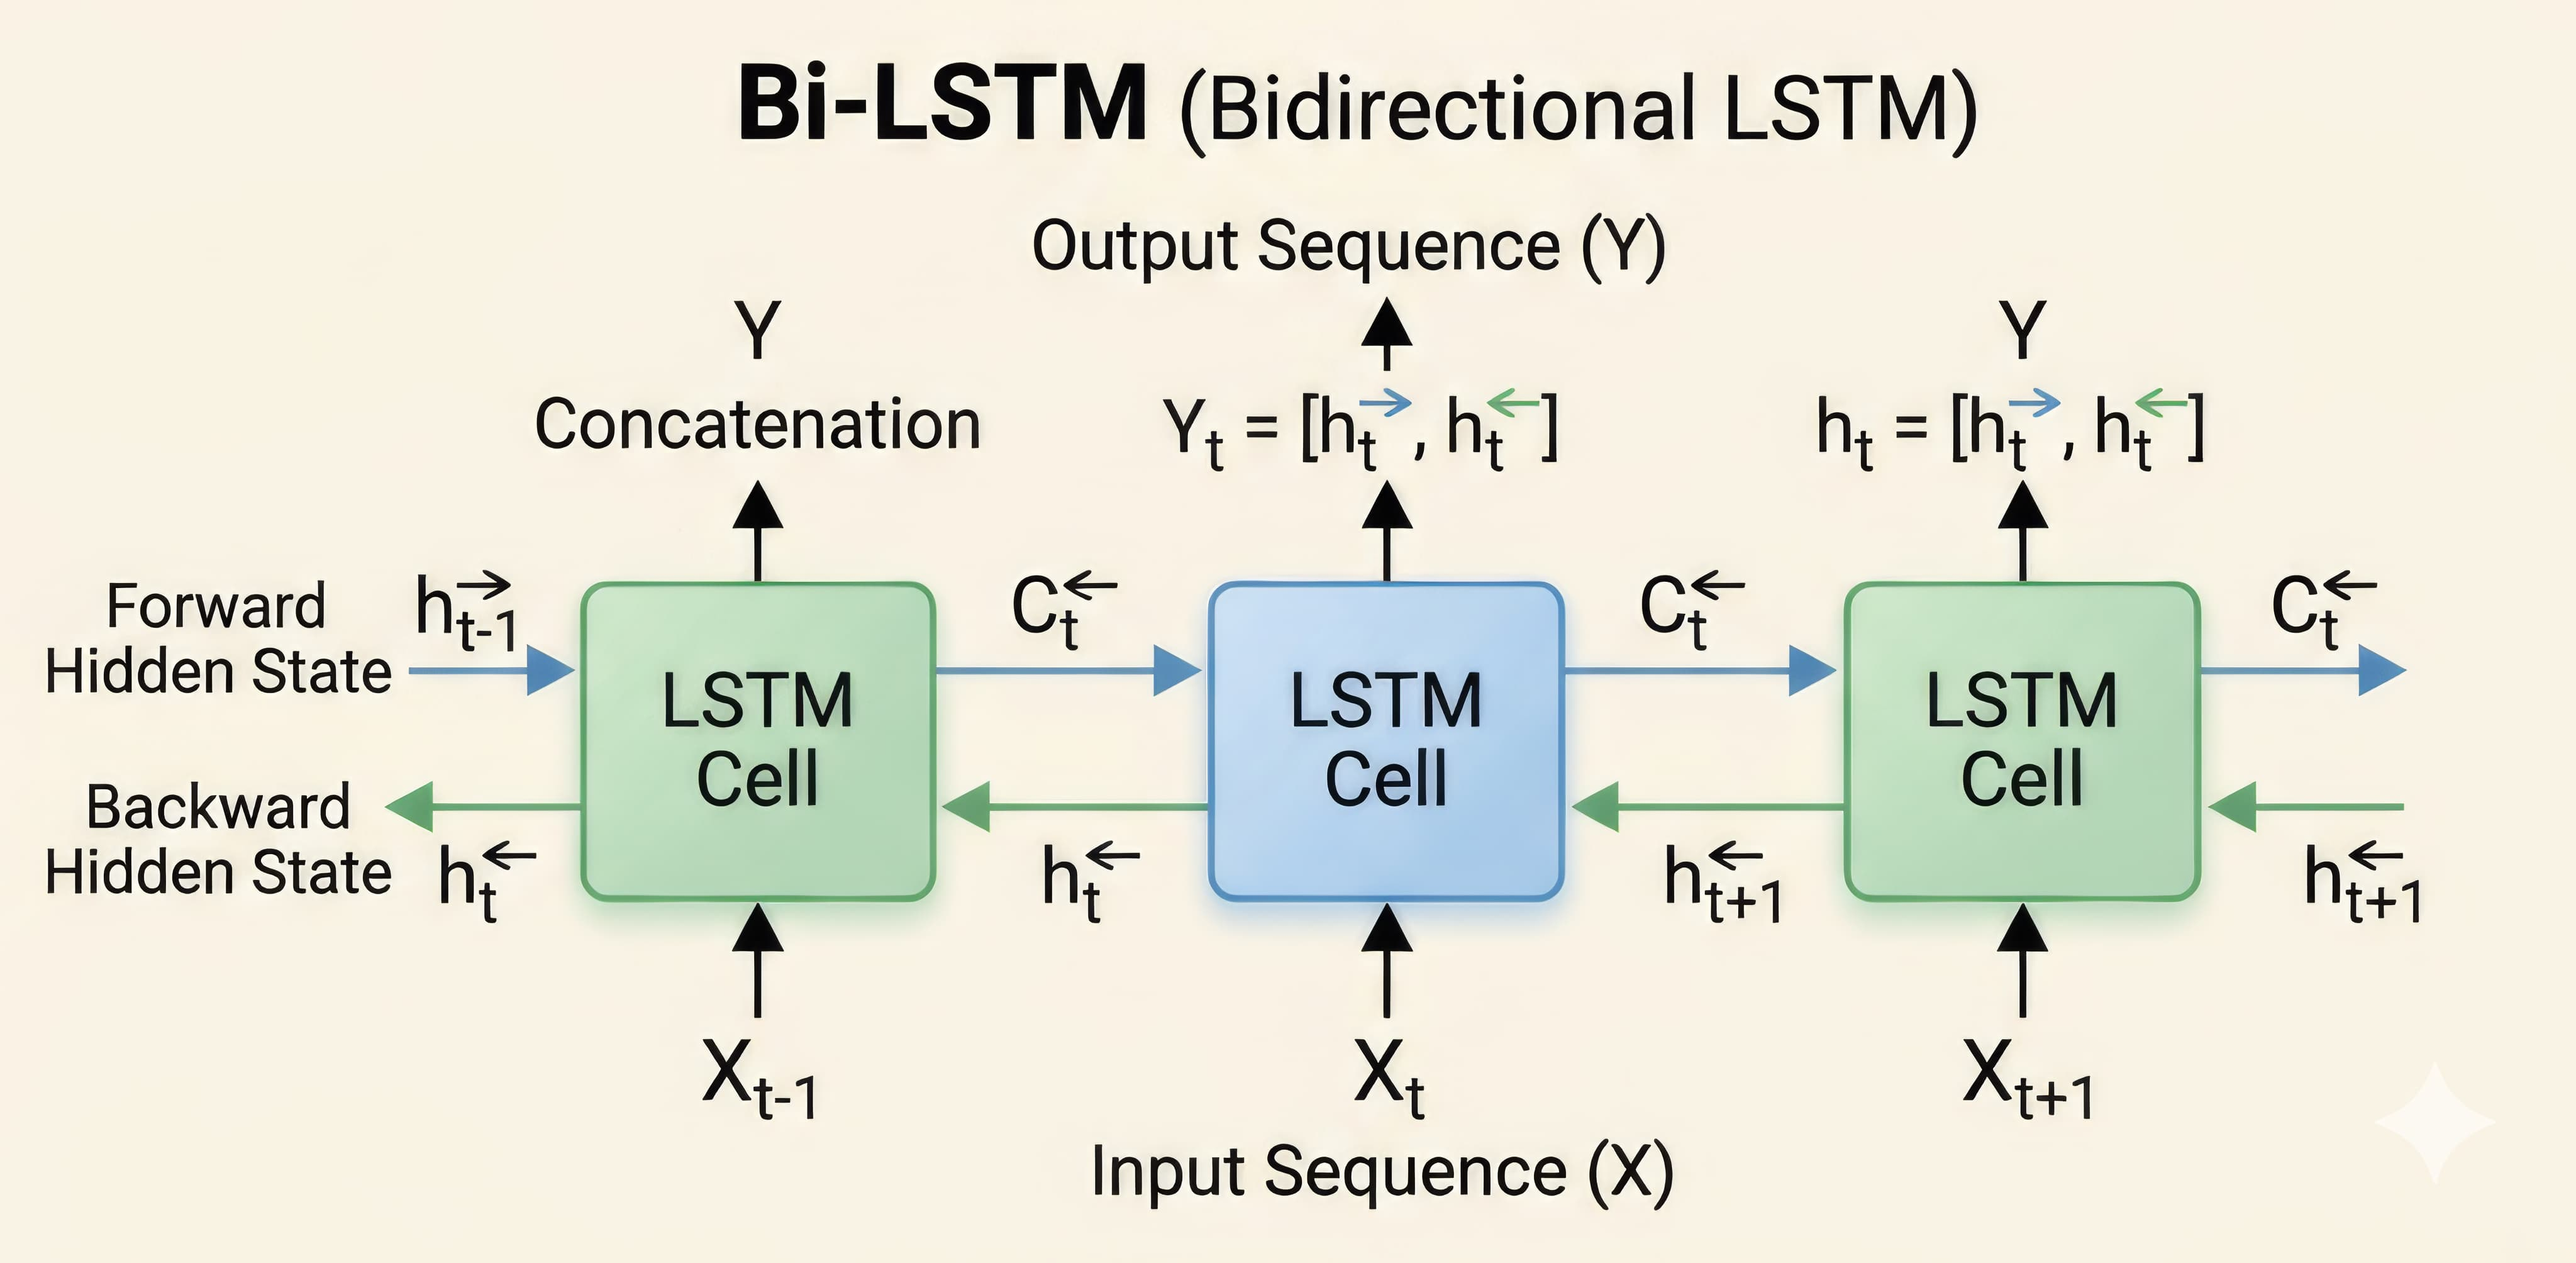
\includegraphics[width=0.9\textwidth]{images/Bi-LSTM.jpg}
    \caption{Cấu trúc của BiLSTM, gồm các cổng điều khiển thông tin.}
\end{figure}

DCNN-BiLSTM kết hợp hai ý tưởng: kiến trúch tích chập để trích xuất mẫu cục bộ và kiến trúc Long-Short Term Memory hai chiều để học phụ thuộc theo hai hướng. Ở phần đầu, dữ liệu đặc trưng được đưa qua lớp Conv1D. Lớp tích chập dùng các bộ lọc trượt trên chuỗi đặc trưng để phát hiện các mẫu cục bộ. Một bộ lọc có thể học rằng một nhóm đặc trưng đứng gần nhau tạo ra tín hiệu hữu ích cho một dạng tấn công. Nhiều bộ lọc khác nhau học nhiều kiểu mẫu khác nhau. Kết quả là mô hình tạo ra một biểu diễn giàu hơn trước khi đưa vào phần hồi tiếp.
\bigbreak\noindent
Sau tích chập, biểu diễn đi vào BiLSTM. LSTM là mạng hồi tiếp có bộ nhớ dài hạn, dùng các cổng để điều khiển thông tin nào được ghi, giữ và xuất ra. BiLSTM chạy LSTM theo hai hướng: một hướng đọc từ đầu đến cuối, hướng còn lại đọc từ cuối về đầu. Hai hướng này được ghép lại để mỗi vị trí trong chuỗi có thông tin từ cả ngữ cảnh trước và sau. Với IDS, cách đọc hai chiều này hữu ích khi ý nghĩa của một đặc trưng phụ thuộc vào cả những đặc trưng đứng trước và đứng sau nó trong biểu diễn đầu vào.
\bigbreak\noindent
Trong lan truyền xuôi, DCNN-BiLSTM hoạt động theo nhiều tầng biểu diễn. Tầng tích chập phát hiện mẫu cục bộ. Tầng BiLSTM thứ nhất giữ chuỗi biểu diễn để học phụ thuộc rộng hơn. Tầng BiLSTM thứ hai nén chuỗi thành một vector ngữ cảnh tổng hợp. Vector này đi qua các lớp dense để tạo biểu diễn phân loại cuối cùng. Layer normalization giúp ổn định biểu diễn, dropout giảm overfitting, còn lớp logits sinh điểm số cho từng lớp.
\bigbreak\noindent
Trong lan truyền ngược, mất mát phân loại truyền gradient qua head dense, qua hai hướng LSTM và về lớp tích chập. Lớp dense học cách dùng biểu diễn tổng hợp để tách lớp. LSTM học cách giữ hoặc quên thông tin theo chuỗi. Lớp tích chập học các bộ lọc cục bộ tốt hơn. Vì nhiều thành phần cùng được cập nhật, DCNN-BiLSTM có năng lực biểu diễn mạnh hơn MLP và GRU. Đổi lại, mô hình có nhiều tham số hơn, chi phí huấn luyện cao hơn và yêu cầu bộ nhớ lớn hơn.
\bigbreak\noindent
Trong bối cảnh IDS, DCNN-BiLSTM phù hợp khi dữ liệu có nhiều tương tác phức tạp và khi hệ thống chấp nhận chi phí tính toán cao để đổi lấy biểu diễn sâu hơn. Trong bối cảnh học liên kết, mô hình này đại diện cho nhóm client mạnh hơn về tài nguyên. Khi đặt cạnh MLP và GRU, nó giúp đánh giá khả năng của các ngữ cảnh mà client không cùng độ phức tạp mô hình. Đây là một điểm quan trọng của học chắt lọc liên kết: các kiến trúc khác nhau vẫn có thể cộng tác thông qua logits hoặc tri thức mềm, thay vì buộc phải có cùng cấu trúc trọng số.

\section{Học máy liên kết}

\subsection{Tổng quan}

Học liên kết là cơ chế huấn luyện phân tán trong đó mỗi client giữ dữ liệu cục bộ và chỉ trao đổi thông tin huấn luyện với server hoặc các client khác. Quy trình cơ bản gồm: server gửi mô hình hiện tại cho client, client huấn luyện cục bộ, client gửi cập nhật, server tổng hợp và phát lại mô hình mới. Mục tiêu là tận dụng dữ liệu phân tán mà không cần chia sẻ dữ liệu thô.

Nếu ký hiệu tham số mô hình ở vòng $t$ là $w^{(t)}$, client $k$ cập nhật $E$ bước với gradient cục bộ $g_k$ thì có thể viết gần đúng
$$
w_k^{(t+1)}=w^{(t)}-\eta\sum_{e=1}^{E} g_{k,e}.
$$
Server sau đó tổng hợp
$$
w^{(t+1)}=\sum_{k=1}^{K}\frac{n_k}{n}w_k^{(t+1)}.
$$

\subsection{FedAvg}

FedAvg là thuật toán nền tảng của học liên kết truyền thống \cite{fedavg}.

FedAvg tổng hợp trọng số mô hình bằng trung bình có trọng số theo số mẫu của client. Đây là thuật toán nền tảng và thường được dùng làm mốc so sánh cho các thuật toán học liên kết khác. Nếu client $k$ có $n_k$ mẫu và tổng số mẫu của các client tham gia là $n=\sum_k n_k$, server cập nhật mô hình toàn cục theo công thức
$$
w^{t+1}=\sum_{k=1}^{K}\frac{n_k}{n}w_k^{t+1}.
$$
Ý nghĩa của công thức này là client có nhiều dữ liệu hơn sẽ đóng góp nhiều hơn vào mô hình toàn cục. Trong môi trường IID, giả định này thường hợp lý vì mỗi client có thể được xem như một mẫu con của cùng một phân phối dữ liệu. Trong môi trường Non-IID, giả định đó yếu đi rõ rệt: một client nhiều mẫu nhưng lệch lớp có thể kéo mô hình toàn cục về phân phối riêng của nó, trong khi một client ít mẫu nhưng chứa lớp hiếm lại có ảnh hưởng nhỏ hơn. Vì vậy, FedAvg đơn giản và hiệu quả, nhưng dễ gặp client drift khi dữ liệu giữa các client không đồng nhất.

\section{Học chắt lọc liên kết}

\subsection{Học chắt lọc}

Chắt lọc tri thức (Knowledge Distillation - KD) \cite{hinton2015kd} là kỹ thuật truyền tri thức từ mô hình này sang mô hình khác thông qua nhãn mềm (soft labels) tính từ phân phối logit và hàm kích họat softmax. Khác với học nhãn cứng như huấn luyện giám sát, mô hình student học phân phối xác suất trong soft labels từ mô hình teacher. Phân phối từ soft labels chứa thông tin về quan hệ giữa các lớp, ví dụ một mẫu có thể rất giống lớp A nhưng cũng gần lớp B hơn các lớp còn lại.

\subsubsection{Temperature và nhãn mềm}

Softmax với temperature $T$ được dùng để làm mềm phân phối xác suất:

$$
p_i = \frac{\exp(z_i / T)}{\sum_j \exp(z_j / T)}.
$$

Khi $T$ lớn hơn, phân phối trở nên mượt hơn và chứa nhiều thông tin hơn về các lớp không phải lớp đúng. Trong chắt lọc tri thức, mô hình học viên thường tối ưu kết hợp giữa mất mát nhãn cứng và mất mát nhãn mềm.

\subsubsection{Chắt lọc bằng Forward Kullback--Leibler}

Phương pháp chắt lọc tri thức được dùng phổ biến nhất dựa trên độ lệch Kullback--Leibler theo chiều thuận giữa hai phân phối softmax: phân phối của mô hình teacher và phân phối của mô hình student. Với logit của giáo viên $z^T$, logit của học viên $z^S$ và temperature $\tau$, hai phân phối mềm được viết là
$$
p_i^T=\frac{\exp(z_i^T/\tau)}{\sum_j\exp(z_j^T/\tau)},
\qquad
p_i^S=\frac{\exp(z_i^S/\tau)}{\sum_j\exp(z_j^S/\tau)}.
$$
Mục tiêu học chắt lọc là làm cho phân phối của student tiến gần phân phối của teacher thông qua mất mát
$$
L_{KD}=\tau^2 KL(p^T\|p^S)=\tau^2\sum_i p_i^T\log\frac{p_i^T}{p_i^S}.
$$
Trong Forward Kullback-Leibler Divergence $KL(p^T\|p^S)$, phân phối giáo viên đuợc đặt ở vai trò tham chiếu, qua đó mô hình student bị phạt thông qua hàm mất mát khi gán xác suất thấp cho những lớp mà mô hình teacher dự đoán khả năng cao. So với mất mát cross-entropy trên nhãn cứng, mục tiêu này truyền thêm "dark knowledge" như quan hệ giữa các lớp: lớp đúng vẫn quan trọng, nhưng các lớp gần với lớp đúng cũng nhận được tín hiệu mềm thay vì bị xem như dự đoán sai trong cross entropy. Trong IDS nhiều lớp, đặc điểm này có ý nghĩa vì nhiều kiểu tấn công có biểu hiện gần nhau, và phân phối mềm giúp mô hình student tiếp nhận cấu trúc trong phân phối mềm mà mô hình teacher đã học được.

\subsubsection{Chắt lọc bằng Evidential Knowledge Distillation}

Evidential Knowledge Distillation (EKD), thay thế phương pháp chắt lọc dựa trên softmax truyền thống là Forward Kullback-Leibler bằng một phân phối Dirichlet trên xác suất lớp \cite{xiang2025ekd,shen2024fdekd}. Với logit $z$, bằng chứng của mô hình được xác định bởi
$$
e=\exp(z),
$$
và tham số Dirichlet được viết là
$$
\alpha=e+\lambda.
$$
Khác với softmax, phép biến đổi theo bằng chứng không loại bỏ hoàn toàn độ lớn tuyệt đối của logit. Tổng nồng độ $\sum_i\alpha_i$ vì vậy trở thành tín hiệu về mức chắc chắn của mô hình: khi bằng chứng lớn và tập trung vào một số lớp, phân phối Dirichlet tập trung tụ lại hơn; khi bằng chứng nhỏ hoặc phân tán, phân phối Dirichlet trải rộng hơn và cho thấy độ bất định cao hơn ở dự đoán của mô hình teacher.

Hàm mất mát của EKD gồm hai thành phần:
$$
L = L_{1st} + \gamma L_{2nd}.
$$
Thành phần thứ nhất căn chỉnh quan hệ tỷ lệ giữa các lớp của học viên và giáo viên:
$$
L_{1st} = KL\!\left(\frac{\alpha_i^T}{\sum_{i \in C}\alpha_i^T} \;\middle\|\; \frac{\alpha_i^S}{\sum_{i \in C}\alpha_i^S}\right).
$$
Thành phần này đóng vai trò chắt lọc ở mức vĩ mô, vì nó tập trung vào hình dạng phân phối lớp sau khi chuẩn hóa. Thành phần thứ hai căn chỉnh toàn bộ phân phối Dirichlet:
$$
L_{2nd} = KL\!\left(Dir(p^T|\alpha^T) \;\middle\|\; Dir(p^S|\alpha^S)\right).
$$
Thành phần này đóng vai trò chắt lọc ở mức vi mô, vì nó giữ lại độ lớn bằng chứng và mức bất định trong phân phối dự đoán của mô hình teacher. Nhờ đó, EKD không chỉ chắt lọc lớp có xác suất cao, mà còn chắt lọc cả mức độ chắc chắn của mô hình khi đưa ra phân phối đó.

\subsubsection{Vai trò trong môi trường liên kết}

Trong học liên kết, chắt lọc tri thức loại bỏ đặc tính đồng nhất kiến trúc. Do các thuật toán học liên kết truyền thống yêu cầu mô hình của các client phải đồng bộ về số chiều để thực hiện tổng hợp, tính thực tiễn của chúng thường bị hạn chế trong các môi trường thực tiễn khi tài nguyên tính toán của mỗi client tham gia rất khác nhau. Mặt khác, chắt lọc kiến thức ban đầu được sử dụng để truyền tải kiến thức giữa các kiến trúc mô hình khác nhau.

Để cho phép các kiến trúc mô hình khác nhau tham gia học liên kết, học máy chắt lọc liên kết chuyển từ tổng hợp trọng số mô hình sang tổng hợp biểu diễn đầu ra của mô hình. Cụ thể hơn, các thuật toán FD sẽ tổng hợp không gian đầu ra như logit vector hoặc prototype theo nhãn, hoặc phân phối dự đoán như logits (có hoặc không có kích hoạt softmax) trên một tập dữ liệu công khai trung gian. Server trong FD sẽ tổng hợp các biểu diễn này và bộ biểu diễn tổng hợp thường được gọi là consensus sẽ đóng vai trò teacher, và mỗi mô hình client sẽ là mô hình student. Thông qua chắt lọc kiến thức từ consensus, FD đạt được tính liên kết giữa các kiến trúc mô hình khác nhau. Điều này đặc biệt phù hợp với IDS vì các tổ chức có thể triển khai mô hình khác nhau tùy tài nguyên và yêu cầu vận hành.

\subsection{FD}

FederatedDistillation \cite{jeong2018federateddistillation} là thuật toán FL tiêu biểu vì thuật toán này dùng nhãn mềm để thay thế cho trao đổi trọng số. Cụ thể, ở mỗi client, mô hình học giám sát và tích lũy soft labels cho từng lớp thành một vector nhãn mềm đại diện cho từng lớp đó $p_{k,c} \leftarrow \frac{1}{|D_{k,c}|\sum_{x \in D_{k,c}}p_k(x)}$. Sau đó, server cộng các vector nhãn mềm này $\bar p_{c} \leftarrow \sum_{k \in K} p_{k,c}$ và mỗi client tự cập nhật mục tiêu chắt lọc bằng cách lấy trung bình bỏ qua chính nó (leave-one-out average):
$$
\bar p_{k,c}=\frac{1}{K-1} (\bar p_c - p_{k,c})
$$

Sau đó, client cập nhật thông qua hàm mất mát chắt lọc. Với mỗi mẫu x thuộc lớp $c$, client tối ưu

$$
L_{FD} = L_{CE} + \lambda KL(\bar p_{k,c} \| p_k(x)).
$$
Với cách này, client không chỉ tự củng cố lại tri thức của chính nó, mà nhận được tín hiệu từ các miền dữ liệu khác. Nếu mục tiêu chắt lọc chứa cả dự đoán của chính client đang học, tín hiệu chung có thể bị kéo về tri thức cục bộ và làm giảm ý nghĩa của việc học liên kết. Leave-one-out average vì vậy làm rõ vai trò của tri thức liên client: mỗi client học từ phần đồng thuận mà các client khác quan sát được trên cùng không gian lớp.

\subsection{FedMD}

FedMD \cite{li2019fedmd} là một thuật toán tiêu biểu khác của hệ thống học chắt lọc liên kết dùng dữ liệu công khai. Ở bước tiền liên kết, mỗi client huấn luyện giám sátn mô hình cục bộ trên tập công khai đã gán nhãn $\{x_p, y_p\} \in D_p$. Sau đó, hệ thống tiến vào giai đoạn học liên kết. Ở mỗi vòng liên kết, client tiếp tục học trên dữ liệu riêng, sau đó dự đoán logit (chưa qua hàm softmax) trên tập công khai, gửi logits tới server để tổng hợp, rồi dùng logit tổng hợp (consensus) này làm mục tiêu chắt lọc:

$$
L_{FedMD} = L_{CE} + \lambda KL(z_{p} \| z_k(x)).
$$

\section{Học liên kết phi tập trung}

\subsection{Động cơ phi tập trung}

Trong học liên kết truyền thống, server trung tâm giữ vai trò điều phối: chọn client, nhận cập nhật của các client tham gia, tổng hợp cập nhật và broadcast kết quả tổng hợp. Cấu trúc này đơn giản nhưng tạo ra một điểm phụ thuộc lớn. Nếu server bị quá tải, bị gián đoạn hoặc không được tất cả tổ chức tin cậy, toàn bộ quá trình học liên kết sẽ bị ảnh hưởng tiêu cực. Học liên kết phi tập trung thay đổi giả định này bằng cách cho phép các client tự điều phối quá trình tổng hợp với nhau mà không cần dựa vào một phần tử cố định.

\subsection{Cơ chế trao đổi trong môi trường phi tập trung}

Nếu ký hiệu $\mathcal{N}(k)$ là tập neighbor (các client kề cạnh trong communication graph) của client $k$, một dạng cập nhật phi tập trung có thể viết là
$$
w_k^{(t+1)}=\sum_{j\in\mathcal{N}(k)}a_{kj}w_j^{(t)},
\qquad \sum_{j\in\mathcal{N}(k)}a_{kj}=1.
$$
Công thức này cho thấy mỗi client tự tổng hợp mô hình mới bằng cách hợp nhất tri thức từ các láng giềng thay vì phải chờ tổng hợp một mô hình toàn cục duy nhất. Khi kết hợp với chắt lọc tri thức, đối tượng trao đổi không nhất thiết là trọng số mô hình $w_j$, mà có thể là logit vector, soft label, prototype hoặc bộ dự đoán trên dữ liệu công khai. Nhờ vậy, thiết kế phi tập trung và chắt lọc tri thức bổ sung cho nhau: phi tập trung cho phép tổng hợp không dựa vào một server, còn chắt lọc kiến thức cho phép tổng hợp kiến thức của nhiều kiến trúc mô hình khác nhau.

\section{Học liên kết tích hợp học tiệm tiến}

\subsection{Học tiệm tiến theo nhãn}

CIL theo dõi khả năng học thêm lớp mới mà vẫn giữ được tri thức cũ. Phần này tập trung vào các thuật toán CIL được dùng làm cơ sở để so sánh với phương pháp đề xuất.

\subsubsection{Bài toán}

CIL mô tả tình huống mô hình học dữ liệu theo từng tác vụ (task), mỗi task $\mathcal{T}$ chứa một tập lớp mới $C^{\mathcal{T}}$. Sau $T$ task, mô hình phải phân loại trên hợp lớp $C^{1:T}=\bigcup_{\mathcal{T}=1}^{T}C^{\mathcal{T}}$ thay vì chỉ phân loại trên lớp mới. Ở task $\mathcal{T}$, dữ liệu đầy đủ của các task trước thường không còn truy cập được, nên mô hình phải học lớp mới trong khi vẫn giữ ranh giới quyết định cho lớp cũ.

Thách thức của CIL là hiện tượng catastrophic forgetting, khi tối ưu theo dữ liệu mới làm tham số rời khỏi vùng từng biểu diễn tốt cho dữ liệu cũ. Có thể nhìn mục tiêu lý tưởng của CIL là tối ưu trên toàn bộ dữ liệu đã từng xuất hiện,
$$
L_{1:T}(w)=\sum_{\mathcal{T}=1}^{T}L_{\mathcal{T}}(w),
$$
nhưng tại thời điểm học task $T$, phần lớn $L_1, L_2, \ldots, L_{T-1}$ không còn được quan sát trực tiếp. Vì vậy, các thuật toán CIL khác nhau chủ yếu khác nhau ở cách giải quyết vấn đề catastrophic forgetting: dùng mô hình cũ làm mô hình teacher và chắt lọc kiến thức task cũ cho mô hình mới, ràng buộc tham số quan trọng, lưu mẫu tái diễn huấn luyện (exemplar), hoặc mở rộng kiến trúc để mô hình thích nghi với lớp mới xuất hiện. Học tiệm tiến theo nhãn như vậy được phân biệt ra $3$ hướng tiếp cận: ràng buộc mô hình thông qua trọng số quan trọng hoặc chắt lọc đầu ra (regularization), tái diễn dữ liệu (exemplar rehearsal/replay) hoặc kiến trúc thích nghi (dynamic architecture). Các hướng này khác nhau ở hàm mất mát, tài nguyên tính toán cũng như yêu cầu về việc biết trước số lượng nhãn.

\subsubsection{Finetune}

Finetune (tối ưu mô hình qua học giám sát) là đường cơ sở cơ bản nhất cho bài toán CIL. Ở task $\mathcal{T}$, mô hình chỉ tối ưu hàm mất mát cross-entropy trên dữ liệu mới:
$$
L_{FT}=L_{CE}(y,p_w(x)),\qquad (x,y)\in D^{\mathcal{T}}.
$$
Không có hạng tử nào ràng buộc trọng số quan trọng, cũng không có bộ nhớ exemplar hoặc mô hình teacher để giúp mô hình mới lưu giữ kiến thức phân loại lớp cũ. Vì vậy, gradient của lớp mới trực tiếp kéo bộ trích xuất đặc trưng (feature extractor) và bộ phân loại (classifier head) về phía phân phối hiện tại. Nếu lớp mới chiếm toàn bộ mini-batch, toàn bộ trọng số mô hình sẽ thay đổi để mang lại hiệu quả phân loại tốt nhất chỉ trên tập lớp mới này. Kết quả là finetune chỉ phân loại tốt trong task mới nhưng thường quên hoàn toàn khả năng phân loại lớp cũ, nên Finetune đóng vai trò cận dưới của bài toán CIL. Trong IDS, đường cơ sở này phản ánh tình huống hệ thống chỉ cập nhật theo kiểu tấn công mới mà không có cơ chế bảo toàn tri thức về những kiểu tấn công đã biết.

\subsubsection{Học tiệm tiến dựa trên ràng buộc mô hình}

\paragraph{Learning without Forgetting - LWF}

\cite{li2017lwf} dùng mô hình cũ làm mô hình teacher để ràng buộc đầu ra của mô hình mới (student) trên các lớp đã học. Ở mỗi task $\mathcal{T}$ và mô hình cũ $w^{old}$, LwF tryền dữ liệu mới đi qua mô hình cũ và mô hình mới, phân phối mềm trên lớp cũ được so khớp bằng chắt lọc tri thức:
$$
L_{LwF}=L_{CE}(y,p_w(x))+
\lambda\tau^2 KL(p_{w^{old}}^{\tau}(x)\|p_w^{\tau}(x)).
$$
Hạng tử đầu học lớp mới bằng nhãn cứng, còn hạng tử thứ hai buộc mô hình mới giữ phản ứng gần với mô hình cũ. Điểm mạnh của LwF là không cần lưu mẫu cũ, nên phù hợp với bối cảnh tài nguyên lưu trữ hạn chế. Tuy nhiên, vì dữ liệu dùng để chắt lọc vẫn là dữ liệu task mới, mô hình cũ chỉ cung cấp tín hiệu cũ thông qua cách nó phản ứng trên mẫu mới. Nếu mẫu mới nằm xa phân phối cũ, phân phối mềm của giáo viên có thể nghèo thông tin và biểu diễn phân phối dự đoán bị sai. Trong IDS, hạn chế này xuất hiện khi kiểu tấn công mới có đặc trưng rất khác các kiểu cũ: mô hình cũ vẫn sinh xác suất trên lớp cũ trong phân phối mềm, nhưng các xác suất đó không đảm bảo đủ tín hiệu để ràng buộc mô hình mới.

\paragraph{Elastic Weight Consolidation - EWC và Memory Aware Synapses - MAS} thuộc nhóm ràng buộc tham số \cite{kirkpatrick2017ewc,aljundi2018mas}. Thay vì lưu mẫu của lớp cũ, nhóm phương pháp này giả định rằng không phải mọi tham số đều quan trọng như nhau đối với tri thức cũ. Nếu một tham số có ảnh hưởng lớn đến phân loại lớp cũ, EWC và MAS ràng buộc thay đổi của nhóm tham số này.

EWC xấp xỉ ảnh hưởng của mất mát cũ quanh nghiệm $w^*$ bằng khai triển bậc hai. Với ma trận Fisher $F_i$, mục tiêu ở task CIL mới được viết là
$$
L_{EWC}=L_{\mathcal{T}}(w)+\frac{\lambda}{2}\sum_i F_i(w_i-w_i^*)^2.
$$
Ở đây $F_i$ đo độ nhạy của log-likelihood cũ theo tham số $w_i$. Nếu $F_i$ lớn, bất cứ thay đổi nào lên tham số đó sẽ bị phạt qua hàm mất mát; nếu $F_i$ nhỏ, biến đổi trên các tham số đó sẽ tạo ra mất mát ít hơn, cho phép mô hình thích nghi nhiều hơn với task mới. Việc điều chỉnh trọng số của hạng tử Fisher $\lambda$ cho góc nhìn rõ ràng hơn về hạn chế stability và plasticity của các phương pháp ràng buộc trọng số: stability đến từ việc giữ tham số quan trọng, còn plasticity đến từ việc vẫn cho phép tham số ít quan trọng học lớp mới, và các siêu tham số như $\lambda$ buộc phải đánh đổi giữa cả hai, từ đó tạo ra hạn chế yêu cầu việc tinh chỉnh tham số trong thực tế.

MAS cũng ràng buộc các thay đổi tham số, nhưng không ước lượng độ quan trọng của tham số dựa trên nhãn hay Fisher information. Phương pháp này đo độ nhạy của chuẩn đầu ra theo tham số:
$$
\Omega_i=\frac{1}{N}\sum_{x}\left\|\frac{\partial \|f(x;w)\|_2^2}{\partial w_i}\right\|.
$$
Mục tiêu học sau đó có dạng
$$
L_{MAS}=L_{\mathcal{T}}(w)+\lambda\sum_i \Omega_i(w_i-w_i^*)^2.
$$
Vì không cần nhãn để ước lượng $\Omega_i$ mà chỉ cần dựa vào thay đổi đầu ra của mô hình, MAS phù hợp hơn khi dữ liệu không được gán nhãn đầy đủ. Trong IDS, hai phương pháp này hữu ích khi không muốn tốn kém chi phí lưu trữ mẫu huấn luyện cũ, nhưng chúng có thể làm mô hình kém linh hoạt nếu kiểu tấn công mới đòi hỏi thay đổi mạnh ở cùng các tham số từng quan trọng cho lớp cũ.

\paragraph{Prototype augmentation and self-supervision for incremental learning - PASS} \cite{zhu2021pass} là phương pháp không dùng exemplar, dựa trên prototype augmentation và self-supervision. Thay vì lưu mẫu cũ, PASS duy trì các prototype của lớp cũ trong không gian đặc trưng. Từ prototype $\phi_c$, phương pháp tạo các đặc trưng giả quanh tâm lớp để mô phỏng vùng dữ liệu cũ:
$$
\tilde \phi_c=\phi_c+\epsilon,\qquad \epsilon\sim\mathcal{N}(0,\sigma_c^2 I).
$$
Các đặc trưng giả này  giúp lớp phân loại của mô hình (classifier head) tiếp tục nhìn thấy tín hiệu của lớp cũ khi học lớp mới. Vì vậy, PASS củng cố decision boundary bằng cách tái tạo vùng lân cận của prototype task cũ thay vì tái tạo mẫu đầu vào. Ngoài ra, tương tự với LwF, PASS hạn chế catastrophic forgetting bằng cách chắt lọc đầu ra của feature extractor cũ cho feature extractor mới ở task mới. Hàm mất mát của PASS như sau:

$$
L_{total} = L_{CE} + \lambda KL(p_{old}(x)\|p_{new}(x)) + \gamma L_{protoAug}.
$$

Trong đó, $\lambda$ và $\gamma$ là hệ số điều chỉnh cho hạng tử chắt lọc và hạng tử huấn luyện classifier head từ đặc trưng giả. $L_{protoAug}$ là hàm mất mát của huấn luyện phân loại các đặc trưng giả $\tilde \phi_c$ vào lớp $c$:

$$
L_{protoAug} = \sum_c L_{CE}(f_{classifier}(\tilde \phi_c), y_c).
$$

trong đó, $f_{classifier}$ là lớp phân loại (classifier head) của mô hình chính $f$, và $f_{classifier}(\tilde \phi_c)$ là đầu ra của lớp phân loại cho đặc trưng giả lớp $c$, còn $y_c$ là nhãn của lớp $c$.

PASS tạo ra một cơ chế chống quên không cần huấn luyện tái diễn: nó không lưu dữ luyện huấn luyện cũ, nhưng vẫn giữ được ước lượng hình học (thông qua prototype) của các lớp đã học.

\paragraph{Correlation-based Knowledge Distillation in Exemplar-Free Class-Incremental Learning - CBKD EFCIL} \cite{gao2025cbkdefcil}. Tương tự như PASS, CBKD EFCIL thuộc nhóm exemplar-free (EF CIL), nghĩa là phương pháp này không lưu mẫu huấn luyện cũ khi chuyển sang task mới. Thay vào đó, CBKD giữ một mô hình cũ làm teacher, một mô hình hiện tại làm student và duy trì prototype của từng lớp trong không gian đặc trưng. Điểm khác biệt chính so với LwF nằm ở cách ràng buộc đầu ra: thay vì chỉ ép hai phân phối xác suất gần nhau bằng KL, CBKD đo mức tương quan giữa phản ứng của mô hình cũ và mô hình mới trên các lớp đã học. Nếu hai vector dự đoán giữ cùng quan hệ tăng giảm giữa các lớp cũ, mô hình mới được xem là còn bảo toàn cấu trúc tri thức cũ tốt hơn, ngay cả khi giá trị logit tuyệt đối đã thay đổi trong quá trình học lớp mới.

Với một mẫu $x$, ký hiệu $\hat q(x)$ là dự đoán của mô hình cũ trên $O$ lớp đã học và $q(x)$ là phần dự đoán tương ứng của mô hình mới. Tương quan Pearson giữa hai vector được tính theo công thức
$$
\rho_{Pearson}(\hat q(x),q(x))=
\frac{\sum_{c=1}^{O}(\hat q_c(x)-\bar{\hat q}(x))(q_c(x)-\bar q(x))}
{\sqrt{\sum_{c=1}^{O}(\hat q_c(x)-\bar{\hat q}(x))^2
\sum_{c=1}^{O}(q_c(x)-\bar q(x))^2}}.
$$
Từ đó, khoảng cách Pearson được viết là
$$
d_{Pearson}(\hat q(x),q(x))=1-\rho_{Pearson}(\hat q(x),q(x)).
$$
Khi hai vector có quan hệ tuyến tính gần nhau, khoảng cách này nhỏ; khi quan hệ giữa các lớp bị đảo hoặc mất tương quan, khoảng cách tăng lên. Vì vậy, hạng tử chắt lọc của CBKD không chỉ giữ xác suất của từng lớp riêng lẻ, mà còn dựa vào tương quan giữa các lớp cũ trong dự đoán của các mô hình (correlation-based).

Với một batch $\mathcal{B}$ gồm $|\mathcal{B}|$ mẫu, CBKD xây dựng hai thành phần tương quan. Thành phần inter-class đo khoảng cách Pearson theo từng mẫu:
$$
L_{inter}=\frac{1}{|\mathcal{B}|}\sum_{i=1}^{|\mathcal{B}|}d_{Pearson}(\hat p_i,p_i),
$$
trong đó $\hat p_i$ và $p_i$ là vector dự đoán trên các lớp cũ của mẫu thứ $i$ từ teacher và student. Thành phần intra-class đo khoảng cách Pearson theo từng lớp cũ trên toàn batch:
$$
L_{intra}=\frac{1}{O}\sum_{j=1}^{O}d_{Pearson}(\hat p^j,p^j),
$$
trong đó $\hat p^j$ và $p^j$ là cột dự đoán của lớp cũ thứ $j$ qua các mẫu trong batch. Hai thành phần này được kết hợp thành mất mát correlation-based feature distillation:
$$
L_{CFD}=\alpha L_{inter}+\beta L_{intra}.
$$
$L_{inter}$ giữ quan hệ giữa các lớp trong từng mẫu, còn $L_{intra}$ giữ cách một lớp cũ phản ứng trên nhiều mẫu khác nhau. Cách kết hợp này phù hợp với CIL vì mô hình mới cần học lớp mới, nhưng vẫn không nên phá vỡ mẫu phản ứng mà mô hình cũ đã học cho các lớp trước.

Bên cạnh chắt lọc tương quan, CBKD duy trì prototype lớp để thay thế cho exemplar. Sau mỗi task, với lớp $c$, prototype được tính bằng trung bình đặc trưng của các mẫu thuộc lớp đó:
$$
\mu_c=\frac{1}{|\mathcal{B}_c|}\sum_{i=1}^{|\mathcal{B}_c|}F(x_i;\theta),
$$
trong đó $F(x_i;\theta)$ là đầu ra của bộ trích xuất đặc trưng và $|\mathcal{B}_c|$ là số mẫu của lớp $c$. Độ phân tán chung của đặc trưng được biểu diễn bằng phương sai $r^2$, tính từ trace của ma trận covariance theo đặc trưng của từng lớp:
$$
r_t^2=\frac{1}{M_{old}+M_{new}}\left(M_{old}r_{t-1}^2+
\sum_{c\in C_t}\frac{\operatorname{Tr}(\Sigma_{t,c})}{D_{proto}}\right),
$$
trong đó $M_{old}$ và $M_{new}$ lần lượt là số lớp cũ được giữ prototype và số lớp mới ở task hiện tại, $C_t$ là tập lớp xuất hiện ở task $t$, $D_{proto}$ là chiều không gian đặc trưng và $\Sigma_{t,c}$ là ma trận covariance của đặc trưng lớp $c$. Từ prototype đã lưu, phương pháp tạo đặc trưng giả bằng nhiễu Gaussian
$$
\xi_c=\mu_c+g r, \qquad g\sim\mathcal{N}(0,I),
$$
rồi đưa $\xi_c$ qua classifier head để huấn luyện phân loại lớp cũ:
$$
L_{proto}=\sum_{c=1}^{O}L_{CE}(C_\phi(\xi_c),y_c).
$$
Như vậy, classifier vẫn tiếp tục nhận tín hiệu về lớp cũ mà không cần lưu exemplar.

Tổng mất mát của CBKD ở các task sau được viết là
$$
L_{CBKD}=L_{CE}+L_{CFD}+\lambda L_{proto}.
$$
Ở task đầu tiên, mô hình chưa có lớp cũ nên chỉ học giám sát và sau đó ghi nhận prototype cho các lớp đã thấy. Từ task thứ hai trở đi, mô hình cũ từ giai đoạn trước cung cấp tín hiệu tương quan trên lớp cũ, còn prototype cục bộ cung cấp dữ liệu đặc trưng giả cho classifier.

\subsubsection{Học tiệm tiến dựa trên tái diễn dữ liệu}

\paragraph{Incremental Classifier and representation learning - iCaRL và Bias Correction - BiC} lưu mẫu exemplar đại diện cho lớp cũ và kết hợp tái diễn dữ liệu (replay) với chắt lọc tri thức \cite{rebuffi2017icarl}. Trong iCaRL, với mỗi lớp $c\in C$, một tập mẫu nhỏ $D^{exemplar}_c$ được chọn sao cho trung bình đặc trưng của exemplar gần trung bình đặc trưng của toàn lớp:
$$
\mu_c=\frac{1}{|D_c|}\sum_{x\in D_c}\phi(x),
\qquad
D^{exemplar}_c\approx \arg\min_D\left\|\mu_c-\frac{1}{|D|}\sum_{x\in D}\phi(x)\right\|.
$$
Khi suy luận, iCaRL dùng nguyên tắc nearest-mean-of-exemplars: mẫu được gán vào lớp có trung bình exemplar gần nhất trong không gian đặc trưng. Trong huấn luyện, exemplar của lớp cũ được trộn với dữ liệu lớp mới, còn chắt lọc tri thức giữ đầu ra của mô hình mới gần mô hình cũ trên các lớp đã học. Vì vậy, iCaRL giải quyết quên bằng hai neo cùng lúc: neo dữ liệu thông qua exemplar và neo hàm thông qua chắt lọc. BiC \cite{wu2019bic} tập trung vào một vấn đề khác của CIL: thiên lệch (bias) về lớp mới. Khi dữ liệu huấn luyện chứa toàn bộ mẫu lớp mới nhưng chỉ một số exemplar lớp cũ, bộ phân loại thường tạo logit lớn hơn cho lớp mới. BiC thêm một tầng hiệu chỉnh tuyến tính lên logits của các lớp mới:
$$
q_c=\alpha z_c+\beta,\qquad c\in C^{\mathcal{T}},
$$
trong đó $z_c$ là logit ban đầu của lớp $c$, còn $\alpha$ và $\beta$ được học để giảm lệch giữa lớp cũ và lớp mới. Ý nghĩa của BiC không nằm ở việc học thêm đặc trưng mới, mà ở việc sửa thang đo đầu ra sau khi mô hình đã học trên dữ liệu mất cân bằng. Trong IDS, cơ chế này quan trọng vì dữ liệu về kiểu tấn công mới thường nhiều hơn trong giai đoạn cập nhật, trong khi các kiểu cũ chỉ còn một số mẫu đại diện hoặc thống kê tóm tắt.

\subsubsection{Học tiệm tiến với kiến trúc dynamic}

Một nghiên cứu tiêu biểu cho nhóm phương pháp này là FOSTER \cite{wang2022foster} dùng cơ chế feature boosting và compression để xử lý mâu thuẫn giữa mở rộng kiến trúc mô hình và giữ kiến trúc mô hình vừa phải để tiết kiệm chi phí tính toán. Ở giai đoạn boosting, mô hình được mở rộng bằng một nhánh biểu diễn mới để học các lớp vừa xuất hiện, trong khi nhánh cũ giữ tri thức đã có. Nếu ký hiệu đặc trưng cũ là $f_{old}(x)$ và đặc trưng mới là $f_{new}(x)$, biểu diễn dùng cho phân loại có thể nhìn như phép ghép
$$
f_{boost}(x)=[f_{old}(x);f_{new}(x)].
$$
Cách ghép này tăng dung lượng biểu diễn, giúp mô hình không phải ép toàn bộ lớp mới vào không gian đặc trưng cũ vốn đã được tổ chức cho các lớp trước. Nhờ vậy, FOSTER giảm áp lực làm biến dạng biểu diễn cũ khi học lớp mới.

Tuy nhiên, nếu cứ mở rộng sau mỗi task, kích thước mô hình sẽ tăng liên tục. Vì vậy, FOSTER dùng giai đoạn compression để nén mô hình mở rộng về một mô hình nhỏ hơn bằng chắt lọc tri thức. Mô hình nén học từ đầu ra hoặc đặc trưng của mô hình đã boost:
$$
L_{comp}=L_{CE}+\lambda KL(p_{boost}^{\tau}\|p_{compact}^{\tau}).
$$
Hai giai đoạn này tách rõ hai nhu cầu của CIL: trước hết cần đủ năng lực để hấp thụ lớp mới, sau đó cần đưa tri thức về một mô hình ổn định để tiếp tục học ở task sau. Trong IDS, FOSTER phù hợp với bối cảnh số lớp tấn công tăng dần, nhưng không thể để mô hình triển khai phình to không kiểm soát sau mỗi lần cập nhật.

% \subsection{Global-Local Forgetting Compensation (GLFC)}

% GLFC \cite{dong2022glfc} là phương pháp FCIL kết hợp bốn cơ chế: exemplar replay, gradient compensating, chắt lọc quan hệ, và lựa chọn mô hình toàn cục tốt nhất qua proxy server. Phương pháp xử lý đồng thời hai nguồn lệch: lệch lớp theo thời gian và Non-IID giữa các client.

% \textbf{Exemplar replay theo herding.}
% Mỗi client $k$ duy trì tập exemplar riêng với ngân sách bộ nhớ $M$ được chia đều cho tất cả các lớp đã quan sát. Exemplar được chọn theo phương pháp herding của iCaRL: với mỗi lớp $c$, đặc trưng của từng mẫu được chuẩn hóa, sau đó các mẫu được chọn tuần tự sao cho trung bình tích lũy của tập đã chọn xấp xỉ gần nhất với trung bình toàn lớp. Khi sang task mới, tập exemplar cũ được thu hẹp để duy trì ngân sách $M$, rồi exemplar cho lớp mới được bổ sung vào. Dữ liệu huấn luyện mỗi vòng gồm mẫu mới lẫn exemplar cũ.

% \textbf{Gradient compensation và relation distillation.}
% Hàm mất mát GLFC gồm hai thành phần. Thành phần thứ nhất, $L_{GC}$, điều chỉnh trọng số per-sample dựa trên sai số dự đoán tại nhãn thật: với mẫu có nhãn $c$, trọng số được tính là $g_i = |\sigma(z_{i,c}) - 1|$, trong đó $z_{i,c}$ là logit tương ứng. Để tránh mất cân bằng giữa nhóm lớp cũ và lớp mới, $g_i$ được chuẩn hóa bằng cách chia cho giá trị trung bình nhóm tương ứng. Thành phần thứ hai, $L_{RD}$, là chắt lọc quan hệ: mô hình cũ tạo ra xác suất sigmoid cho $C_{old}$ lớp đã học, các xác suất này được ghép với nhãn thật của lớp mới để tạo tín hiệu chắt lọc. Tổng hàm mất mát:
% $$
% L_{GLFC} = \tfrac{1}{2}\,L_{GC} + \tfrac{1}{2}\,L_{RD}.
% $$
% Khi chưa có lớp cũ (task đầu tiên), $L_{RD} = 0$ và chỉ có $L_{GC}$ được tối ưu.

% \textbf{Gradient encoder và gradient masking.}
% GLFC tích hợp một cơ chế tùy chọn để hỗ trợ lựa chọn mô hình tốt nhất qua máy chủ trung gian (proxy server). Mỗi client huấn luyện một mạng encoder $E_\theta$ nhỏ (dense hoặc GRU hai lớp với đầu ra $C$ lớp) để mã hóa thông tin prototype lớp. Với mỗi lớp mới $c$, client chọn mẫu trung tâm $\mathbf{x}^*_c$ (mẫu gần nhất với trung bình đặc trưng chuẩn hóa của lớp đó), sau đó tinh chỉnh nhẹ $\mathbf{x}^*_c$ bằng SGD và hàm mất mát sigmoid cross-entropy để tăng cường tính đại diện. Tiếp theo, gradient của $E_\theta$ tại mẫu tinh chỉnh đó được tính và làm thưa bằng cách đặt về 0 tất cả phần tử có giá trị tuyệt đối dưới phân vị thứ 30. Tập gradient có mặt nạ này được gửi đến proxy server thay vì gửi dữ liệu thô, nhờ đó bảo vệ quyền riêng tư.

% \textbf{Tái tạo dữ liệu bằng DLG và lựa chọn mô hình.}
% Proxy server nhận tập gradient $\{G_j\}$ từ các client, suy ra nhãn lớp cho mỗi $G_j$ từ cột có gradient âm lớn nhất trong lớp fully-connected cuối, rồi tái tạo mẫu dữ liệu giả thông qua Deep Leakage from Gradients (DLG) \cite{zhu2019dlg}. Cụ thể, với mỗi gradient $G_j$, một biến $\tilde{\mathbf{x}}$ được khởi tạo ngẫu nhiên và tối ưu bằng Adam để gradient của $E_\theta$ tại $\tilde{\mathbf{x}}$ xấp xỉ $G_j$:
% $$
% \tilde{\mathbf{x}}^* = \arg\min_{\tilde{\mathbf{x}}} \sum_l \bigl\|\nabla_{\theta_l} \mathcal{L}(E_\theta(\tilde{\mathbf{x}}), c_j) - G_j^{(l)}\bigr\|^2.
% $$
% Các mẫu tái tạo được tích lũy thành tập proto-data của proxy server. Sau mỗi vòng tổng hợp, proxy server đánh giá mô hình toàn cục trên tập proto-data này và chỉ lưu lại trọng số của mô hình nào đạt độ chính xác cao nhất. Trước khi bắt đầu task tiếp theo, trọng số tốt nhất đó được dùng để khởi tạo mô hình cũ $f_{old}$ thay vì dùng trọng số từ vòng cuối, giúp $L_{RD}$ chắt lọc từ một mô hình ổn định hơn.

\subsection{Federated Geometry-Aware Correction} \cite{qi2026feat} FEAT là một hệ thống học liên kết tích hợp học tiệm tiến khai thác cấu trúc hình học của không gian đặc trưng thông qua Equiangular Tight Frame (ETF). Khác với các phương pháp dựa vào replay hoặc chắt lọc đầu ra, FEAT thay thế classifier head bằng một ma trận prototype tĩnh có cấu trúc ETF, từ đó kiểm soát hình học của biểu diễn lớp ngay tại tầng cuối.

Giả sử tại task $t$, tập lớp tích lũy là $C_t$ với $|C_t|$ lớp, và bộ trích xuất đặc trưng sinh ra biểu diễn $f(x) \in \mathbb{R}^d$. FEAT xây dựng ma trận ETF $W_t \in \mathbb{R}^{d \times |C_t|}$ sao cho mỗi cột $\phi_c$ là prototype chuẩn hóa của lớp $c$ và thỏa mãn
\[
\phi_i^{\top} \phi_j =
\begin{cases}
1, & i=j,\\
\dfrac{-1}{|C_t|-1}, & i\neq j.
\end{cases}
\]
Cấu trúc này đảm bảo mọi prototype có cùng chuẩn $\ell_2$ và góc giữa hai lớp bất kỳ là đồng đều, nhờ đó giảm bias hình học giữa các lớp cũ và lớp mới.

Logit của mẫu $x$ được tính trực tiếp bằng tích vô hướng
\[
z_c = f(x)^{\top} \phi_c,
\]
và mất mát phân loại được viết là
\[
L_{CLS} = - \sum_{c \in C_t} y_c \log \operatorname{softmax}(f(x)^{\top} \phi_c).
\]
Ở task đầu tiên, $L_{CLS}$ là thành phần duy nhất. Từ task thứ hai trở đi, FEAT bổ sung hạng tử Geometric Structural Alignment (GSA):
\[
L = L_{CLS} + \lambda L_{GSA}.
\]

Với một batch $B \subset D$ có $|B|$ mẫu, ký hiệu $f_a = f(x_a)$ là đặc trưng của mẫu $a$. Ma trận tương đồng đặc trưng được tính bằng cosine similarity
\[
M_F^{a,b} = \frac{\langle f_a, f_b \rangle}{\|f_a\|_2 \|f_b\|_2}.
\]
Ma trận mục tiêu $M_P$ được xây dựng từ các prototype ETF tương ứng với nhãn của từng mẫu:
\[
M_P^{a,b} = \frac{\langle \phi_{y_a}, \phi_{y_b} \rangle}{\|\phi_{y_a}\|_2 \|\phi_{y_b}\|_2}.
\]
Sau khi chuẩn hóa từng hàng bằng softmax để thu được phân phối $P_F^a$ và $P_P^a$, mất mát GSA được tính bằng
\[
L_{GSA} = \frac{1}{|C_{batch}|} \sum_{c \in C_{batch}} \frac{1}{|D_c \cap B|} \sum_{a: y_a = c} KL(P_F^a \| P_P^a).
\]
Hạng tử này buộc cấu trúc tương đồng giữa các mẫu trong không gian đặc trưng tiệm cận cấu trúc simplex đều của ETF. Việc lấy trung bình theo từng lớp trước khi lấy trung bình trên các lớp cũng giúp giảm ảnh hưởng của mất cân bằng lớp trong batch.

Để xử lý drift giữa nhóm lớp mới (head) và lớp cũ (tail), FEAT chia $W_t$ thành hai phần $W_H$ và $W_T$ tương ứng với $C_H$ và $C_T$. Từ đó, hai projector được xây dựng bằng Moore--Penrose pseudoinverse:
\[
P_H = W_H (W_H^{\top} W_H)^{\dagger} W_H^{\top}, \qquad
P_T = W_T (W_T^{\top} W_T)^{\dagger} W_T^{\top}.
\]
Với đặc trưng chuẩn hóa $\tilde f$, năng lượng chiếu được định nghĩa là
\[
e_H(\tilde f) = \frac{\|P_H \tilde f\|_2^2}{|C_H|-1}, \qquad
e_T(\tilde f) = \frac{\|P_T \tilde f\|_2^2}{|C_T|-1}.
\]
Trong giai đoạn exemplar replay, mỗi client $k$ tính trung bình trượt (EMA) của hai năng lượng này trên tập exemplar $D_{k,T}$:
\[
e_{H,k} \leftarrow (1-\rho)e_{H,k} + \rho\frac{1}{|D_{k,T}|}\sum_{x \in D_{k,T}} e_H(\tilde f(x)),
\]
\[
e_{T,k} \leftarrow (1-\rho)e_{T,k} + \rho\frac{1}{|D_{k,T}|}\sum_{x \in D_{k,T}} e_T(\tilde f(x)).
\]
Server tổng hợp theo số mẫu để thu được prior toàn cục
\[
\bar e_H^{(G)} = \frac{\sum_k |D_{k,T}| e_{H,k}}{\sum_k |D_{k,T}|}, \qquad
\bar e_T^{(G)} = \frac{\sum_k |D_{k,T}| e_{T,k}}{\sum_k |D_{k,T}|}.
\]

Ở pha suy luận, với đặc trưng chuẩn hóa $\tilde x$, FEAT xây dựng hệ số điều chỉnh
\[
g(\tilde x) = \max \left\{ \frac{e_H(\tilde x) - \bar e_H^{(G)}}{e_H(\tilde x) + e_T(\tilde x) + \varepsilon}, 0 \right\},
\]
rồi hiệu chỉnh biểu diễn bằng cách giảm thành phần head-aligned và tăng thành phần tail-aligned:
\[
\tilde x' = \tilde x - g(\tilde x) P_H \tilde x + g(\tilde x) P_T \tilde x,
\qquad
\tilde x' \leftarrow \frac{\tilde x'}{\|\tilde x'\|_2}.
\]
Dự đoán cuối cùng được tính bằng ETF similarity:
\[
z_c = (\tilde x')^{\top} \phi_c, \qquad c \in C_t.
\]

% Nhờ cấu trúc ETF và cơ chế hiệu chỉnh dựa trên năng lượng chiếu, FEAT không chỉ duy trì exemplar replay như iCaRL, mà còn kiểm soát hình học của không gian đặc trưng trong suốt quá trình học tiệm tiến liên kết. Điều này phù hợp với FCIL trong IDS, nơi mỗi client có thể quan sát phân phối lớp khác nhau và lớp mới xuất hiện dần theo thời gian.

Nhờ cấu trúc ETF và cơ chế hiệu chỉnh dựa trên năng lượng chiếu, FEAT không đơn thuần là exemplar rehearsal như iCaRL mà còn chủ động bảo toàn cấu trúc hình học của không gian đặc trưng trong suốt quá trình học tiệm tiến liên kết. Điều này đặc biệt phù hợp với bài toán FCIL trong IDS, nơi dữ liệu giữa các client thường không đồng nhất, các lớp tấn công mới xuất hiện theo thời gian và mô hình cần thích nghi liên tục mà không làm suy giảm đáng kể khả năng nhận diện các lớp đã học trước đó.

